\documentclass[aspectratio=169]{beamer}
\usepackage[utf8]{inputenc}
\usepackage[T1]{fontenc}
\usepackage{calc}
\usepackage{adjustbox}
\usepackage[absolute,overlay]{textpos}
\usepackage{graphicx}


% for medcirc/medbullet
\usepackage{txfonts}
\usepackage{pxfonts}

% for video
\usepackage{multimedia}
\usepackage{easter}
\usepackage{xcolor}

\setbeamertemplate{blocks}[rounded]
% \setbeamertemplate{blocks}[rounded]

% I don't like the navigations menu
\beamertemplatenavigationsymbolsempty

% footer
\setbeamertemplate{footline}
{%
  \hspace{2em}
    Andreas  
\includegraphics[height=.9em]{./figures/hare_head_darkmode.pdf} \#EH22
  \hspace*{\fill}
    \insertframenumber/\inserttotalframenumber
  \hspace{2em}
  % space to bottom border
  \vskip10pt
}

% bunnify itemize
\setbeamertemplate{itemize item}{
\includegraphics[height=.9em]{./figures/hare_head_darkmode.pdf}}

\begin{document}

\begin{frame}{}
    \centering
    
\includegraphics[width=.7\textwidth]{figures/logo_easterhegg.png}\\
    ROS for everyone!
    \vspace{1em}\\
    Andreas Bresser\\
    \tiny{
    \textit{\url{https://mastodon.social/@brean}}\\
    \textit{\url{https://github.com/brean/}}}
\end{frame}

\begin{frame}{Why am I giving this talk?}
        \centering
        \begin{columns}
            \column{0.3\textwidth}
                \movie[height=0.3\textheight, loop, autostart=true] {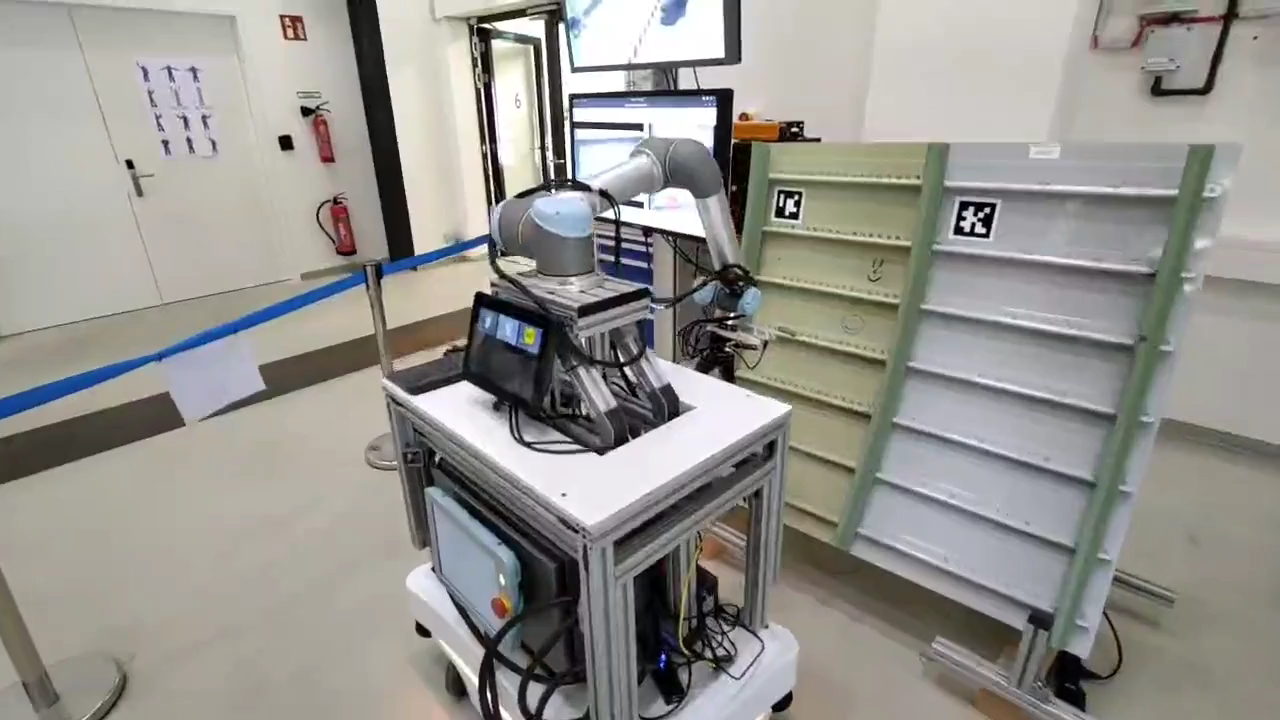
\includegraphics[height=0.3\textheight]{video/semosys_mobipick.png}}{video/semosys_mobipick.mp4}

            \column{0.3\textwidth}
                \movie[height=0.3\textheight, poster, loop, autostart=true] {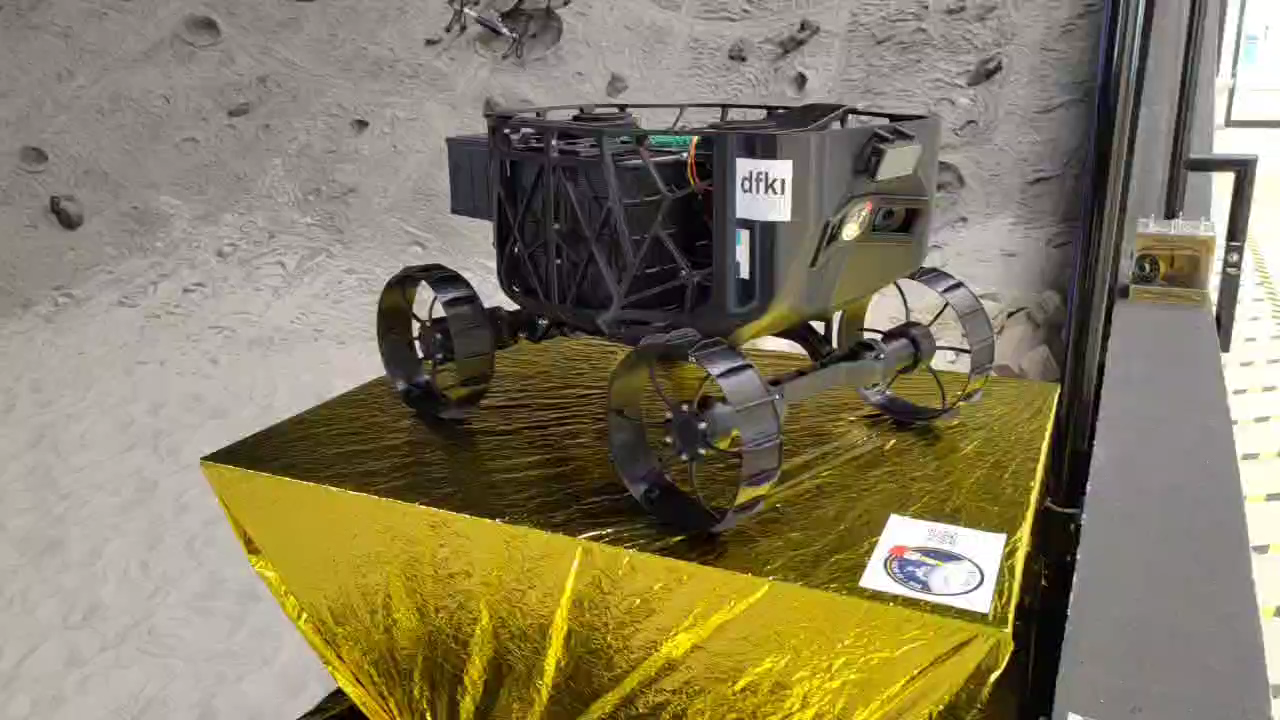
\includegraphics[height=0.3\textheight]{video/samler_robot.png}}{video/samler_robot.mp4}
            \column{0.3\textwidth}
                \movie[height=0.3\textheight, poster, loop, autostart=true] {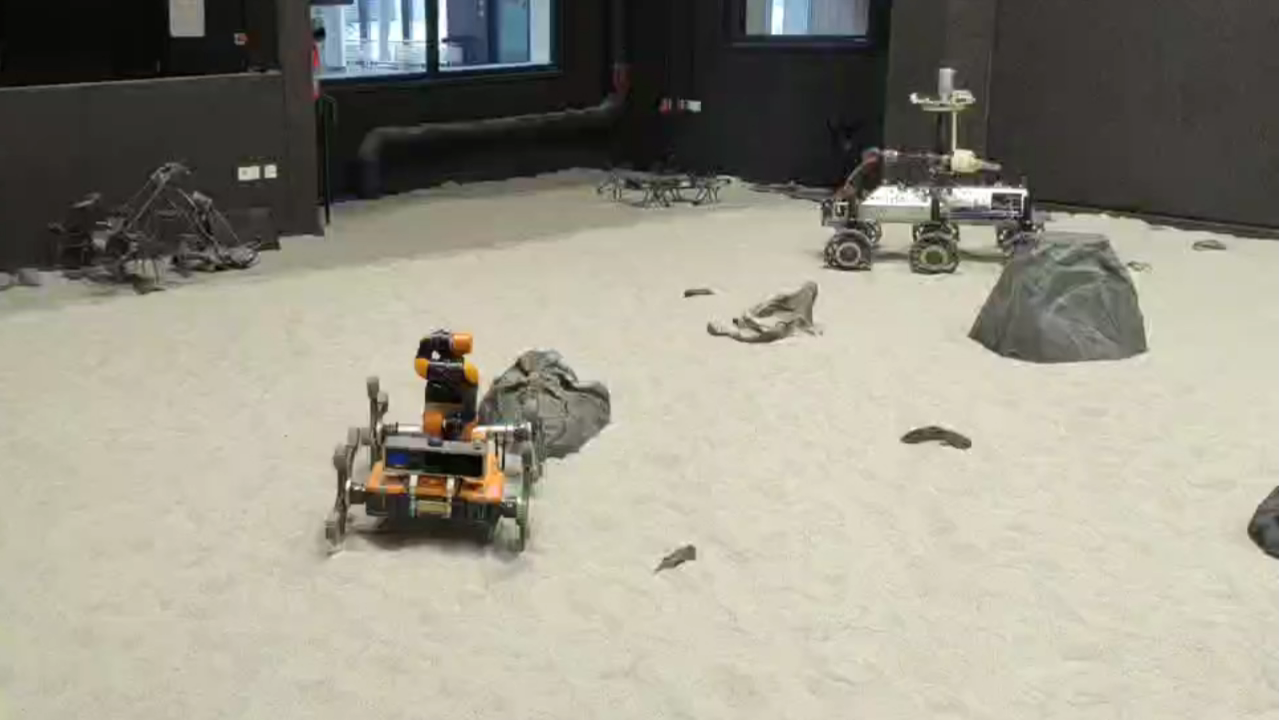
\includegraphics[height=0.3\textheight]{video/coyote.png}}{video/coyote.mp4}
        \end{columns}
        \vspace{1.5em}
        I work with robots!\\
        \textit{(and I like to see more robots at Chaos 
\includegraphics[height=1em]{figures/hare_head_darkmode.pdf} events)}
\end{frame}

\begin{frame}{I love space robotics competitions!}
  \begin{columns}
    \column{0.5\textwidth}
      \centering
      I am part of the DFKI and DLR team BREMEN for the
      ESA SPACE RESOURCES CHALLENGE\\ (13-17. October 2025)\\
      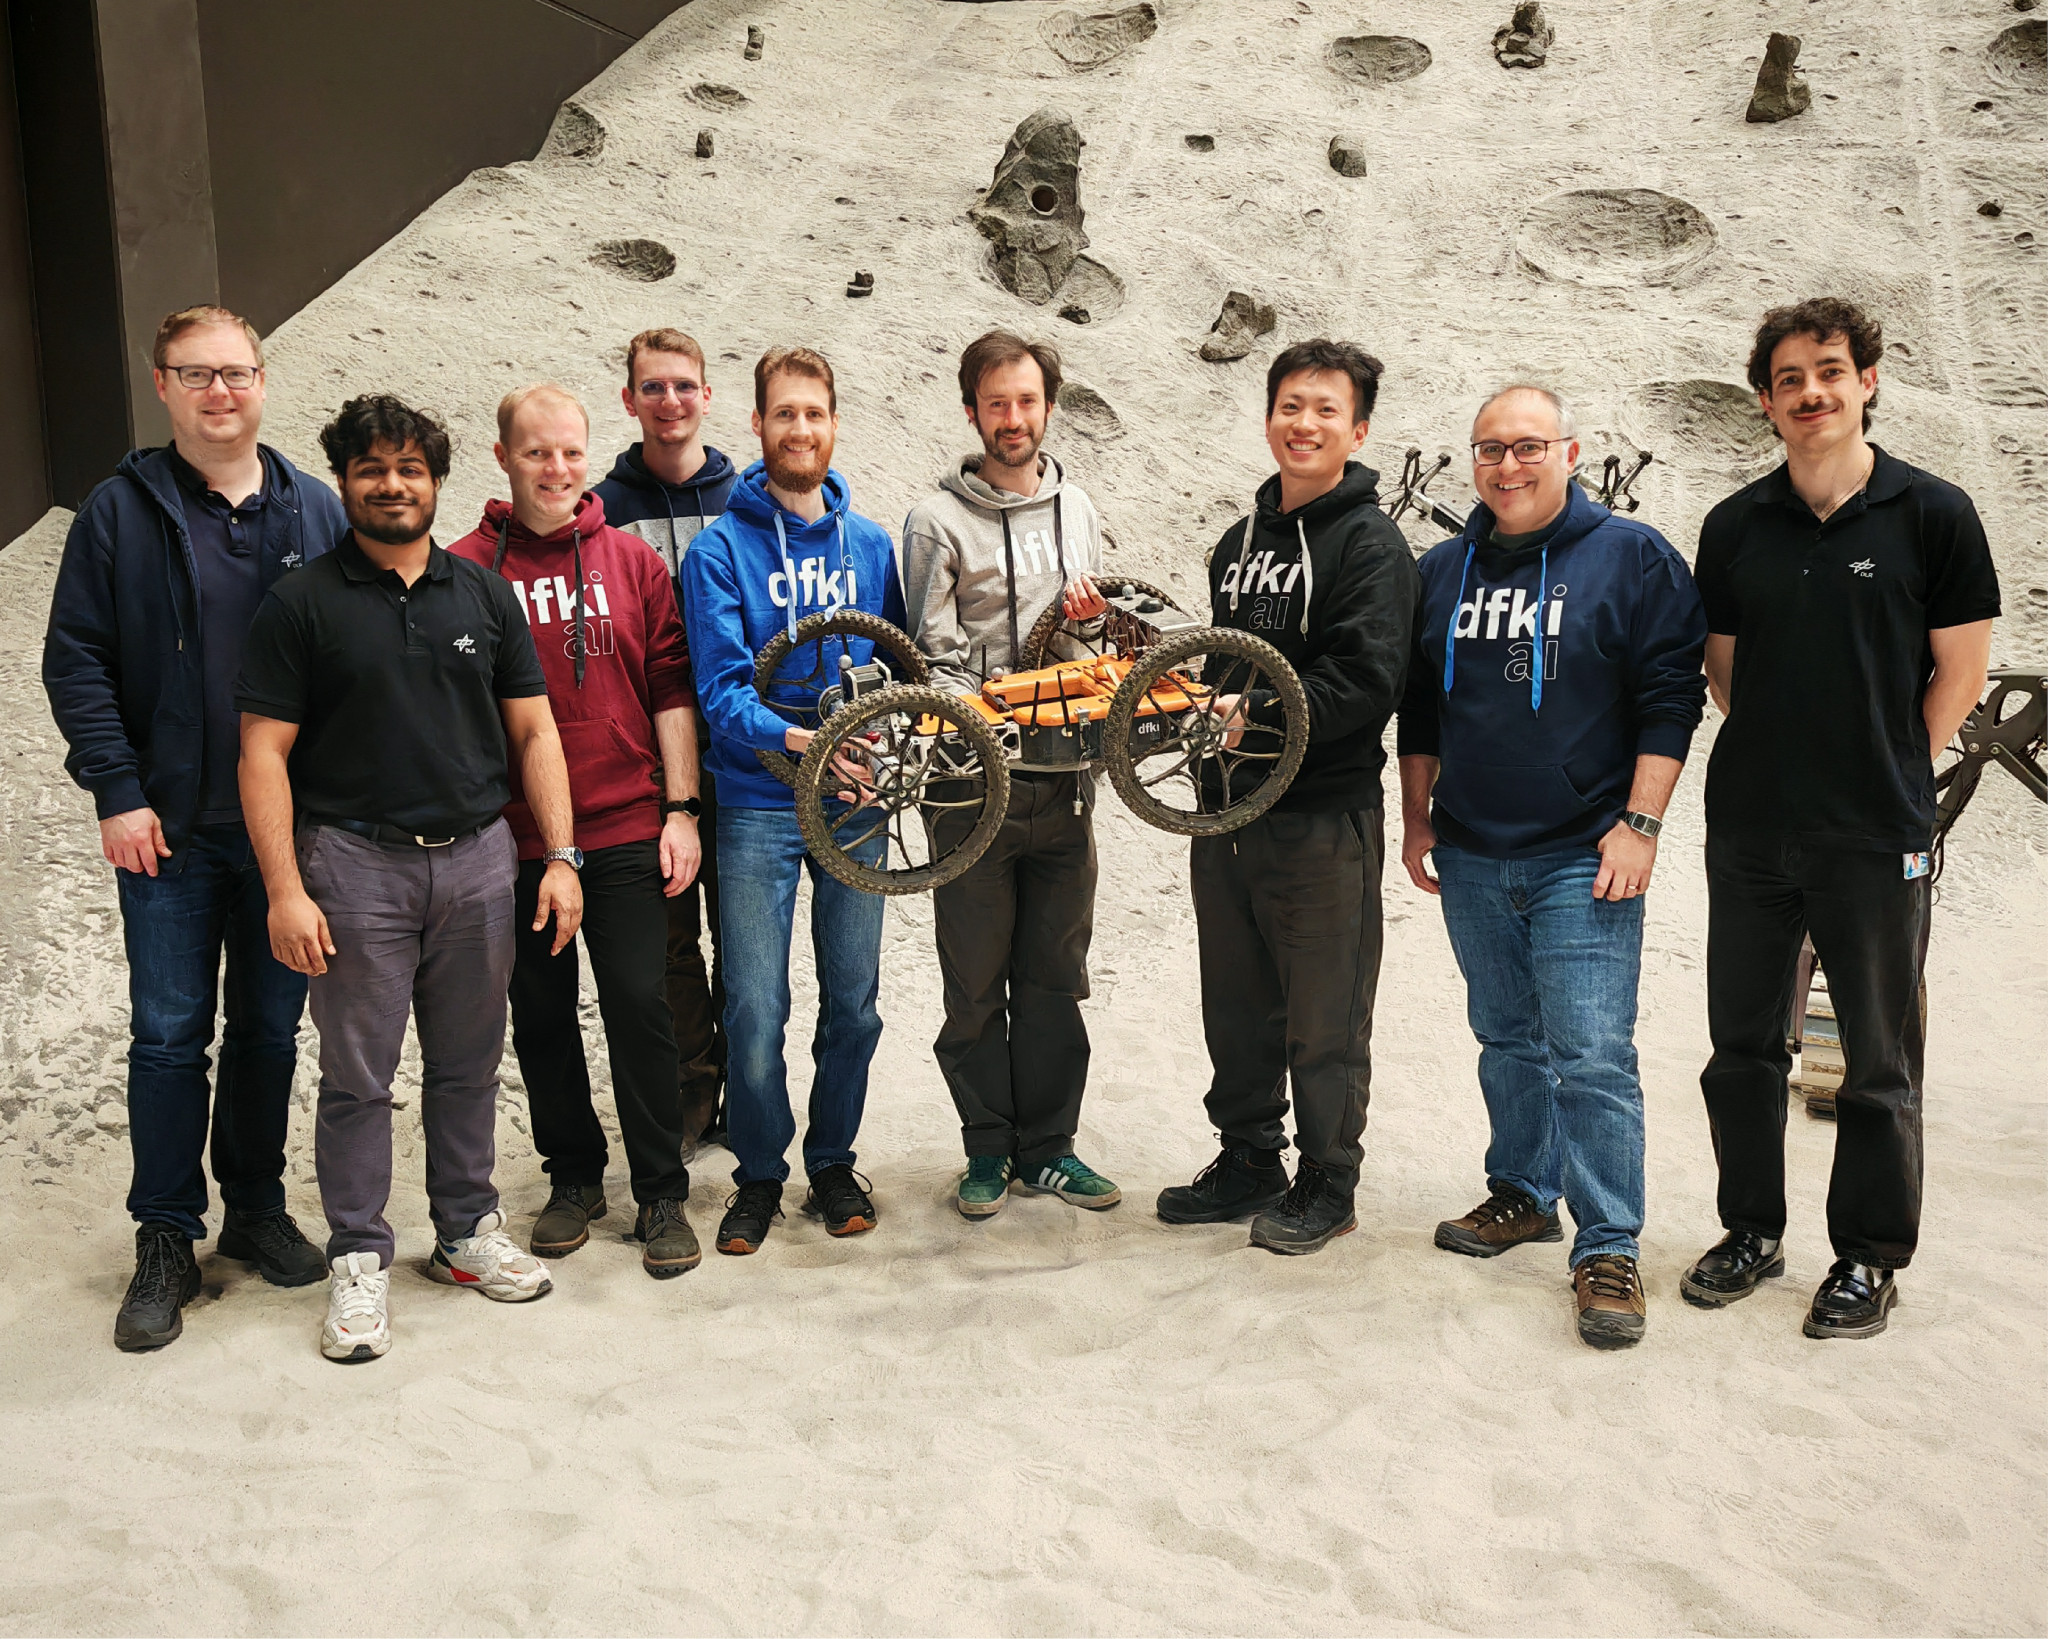
\includegraphics[width=0.8\textwidth]{figures/esasrc-team-bremen.jpg}
    \column{0.5\textwidth}
    \centering
      I am supervising the student team BIRD for the
      European Rover Challenge (29-31 August 2025)
      
\includegraphics[width=0.8\textwidth]{figures/European-Rover-Challenge-logo.pdf}
      
\includegraphics[width=0.8\textwidth]{figures/bird.pdf}
  \end{columns}
\end{frame}

\begin{frame}{Topology}{Topology of a Robot}
    \begin{block}{The Robotics problem...}
      \begin{columns}
        \column{0.45\textwidth}
          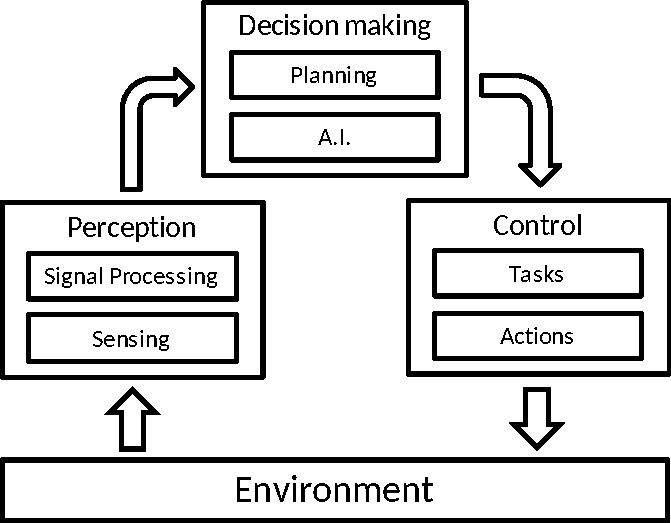
\includegraphics[width=6.6cm]{figures/topology.pdf}
        \column{0.5\textwidth}
          Distributed processes:
          \begin{itemize}
            \item Sensor data sampling
            \item Data/signal processing
            \item Decision making
            \item Control signals $\rightarrow$ actuators
          \end{itemize}
      \end{columns}
    \end{block}
  \end{frame}

\begin{frame}{What is ROS}
    \begin{block}{\textbf{Not} an Operating System but a \textbf{Middleware}}
        
\includegraphics[width=\textwidth]{figures/ros-equation.pdf}
    
        \hfill \tiny{Image source: \url{https://www.ros.org/blog/ecosystem/}}
      \end{block}
\end{frame}

\begin{frame}{Nodes}{What is a ROS Node?}
    \textbf{Nodes are processes.}\\
      A \textbf{node} is a small program that should be responsible for a single, module purpose. 
      Examples of nodes:    
      \begin{figure}[tbh!]
          \centering
        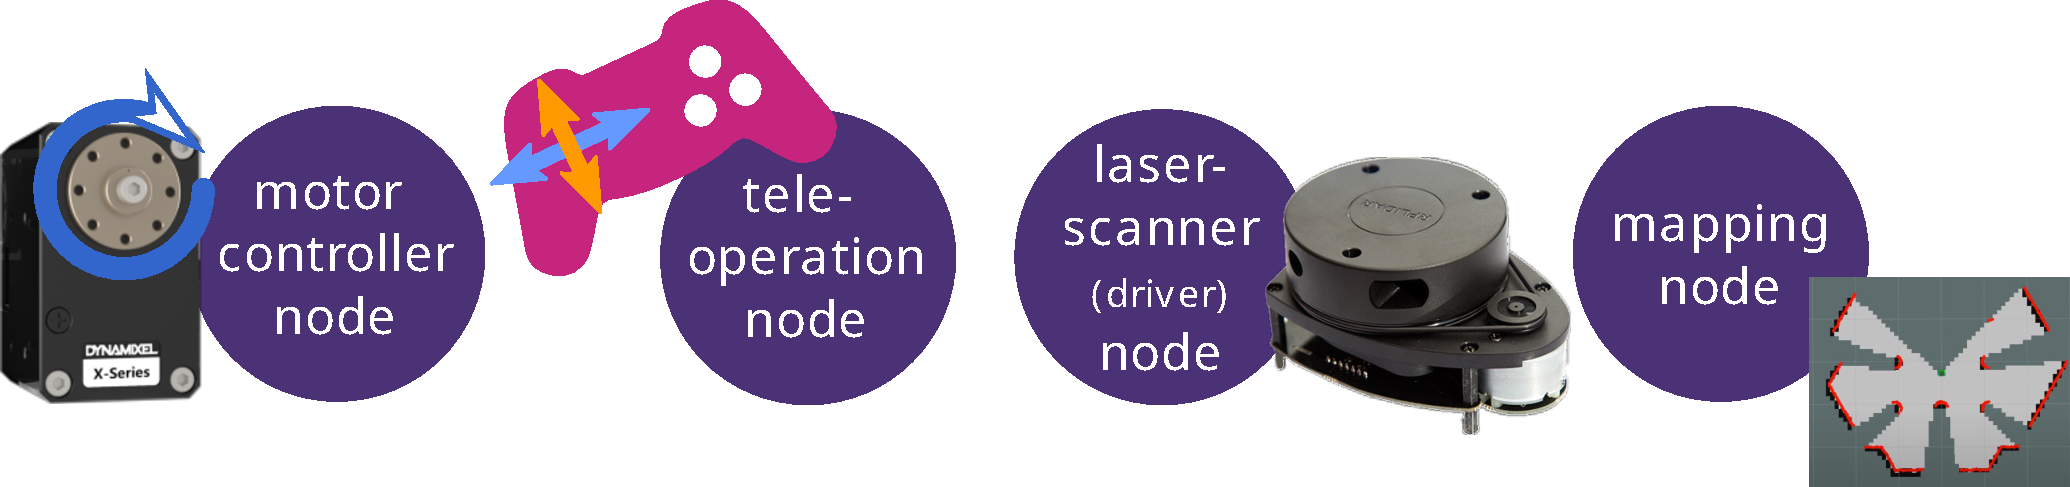
\includegraphics[width=.75\textwidth]{./figures/nodes.pdf}
      \end{figure}
      Nodes are normally written in Python or C++.
    % https://docs.ros.org/en/foxy/Tutorials/Understanding-ROS2-Nodes.html
\end{frame}
  
  \begin{frame}{Nodes}{What is a ROS Node?}
    \textbf{Where are the nodes running?}\\
      \begin{figure}[tbh!]
        \centering
        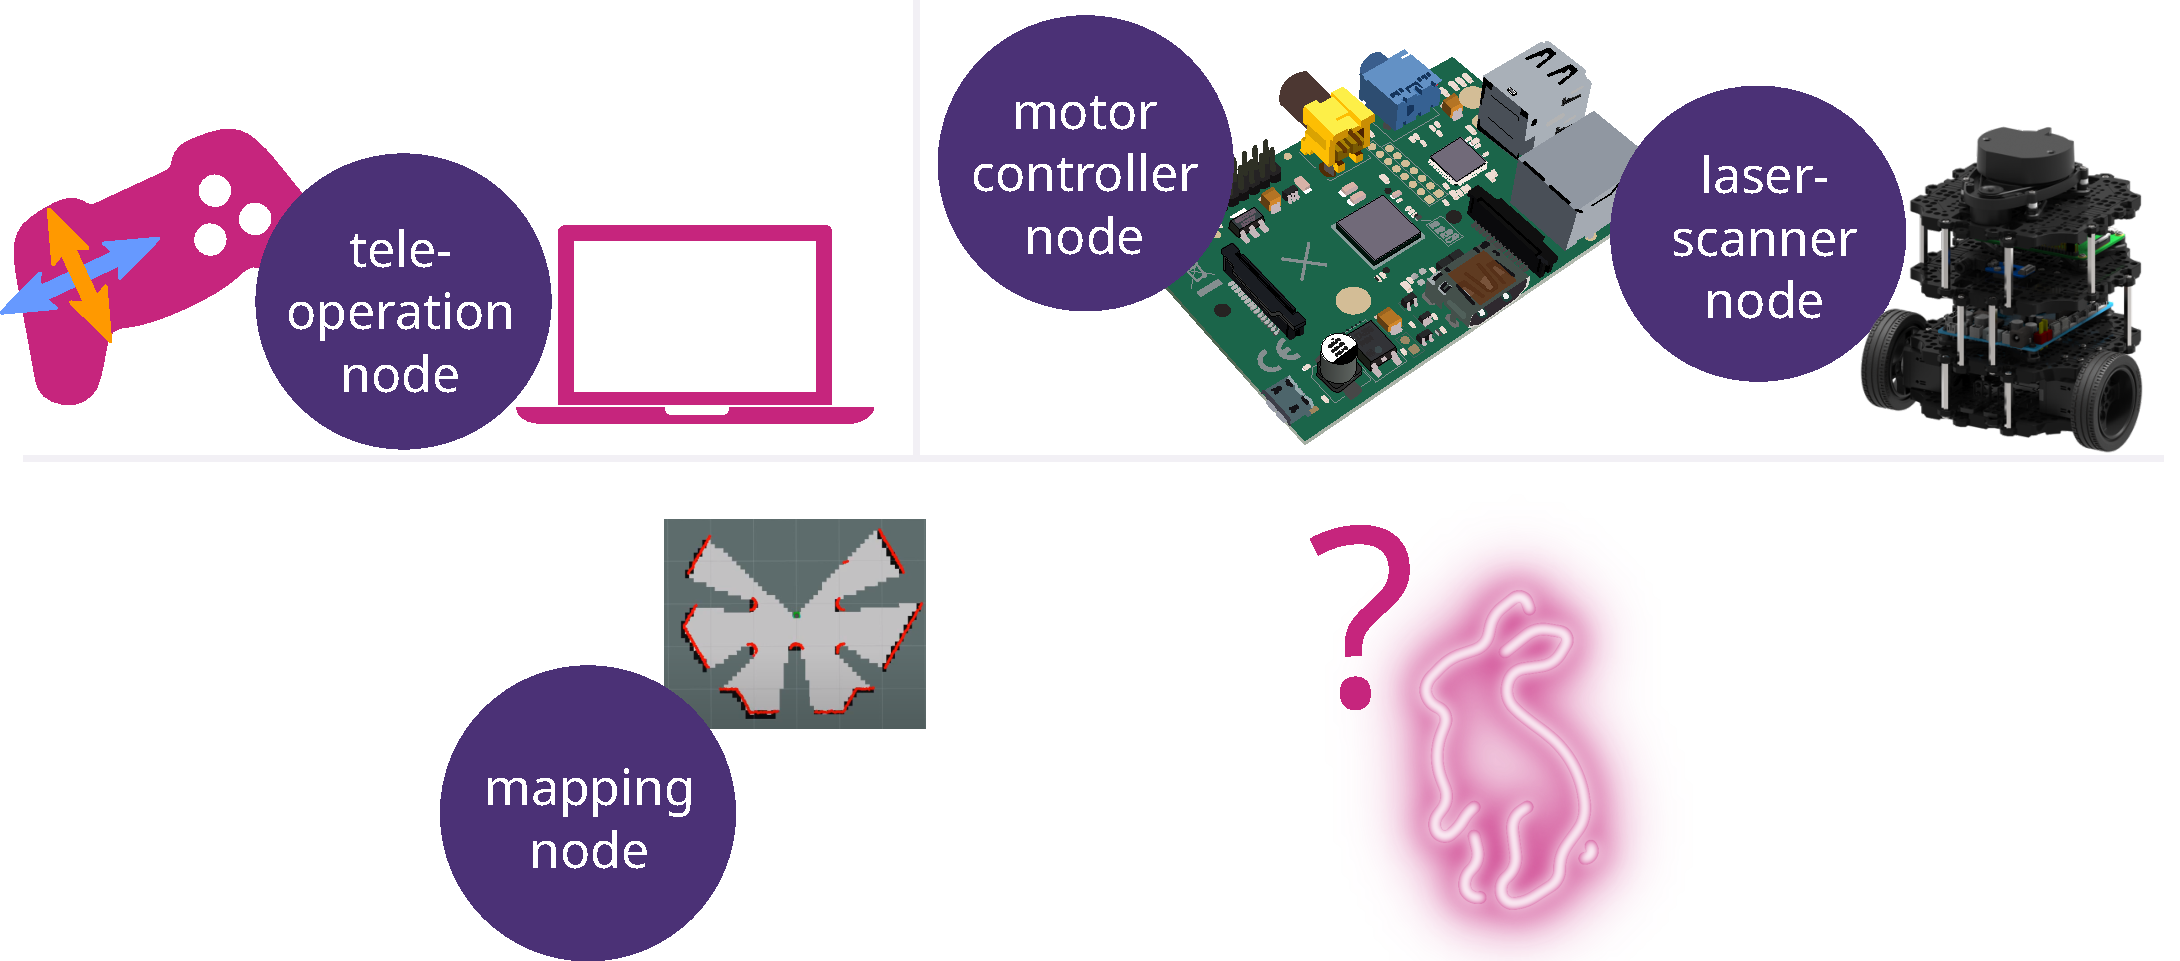
\includegraphics[width=.9\textwidth]{./figures/where_should_a_node_run.pdf}
      \end{figure}
  \end{frame}

\begin{frame}[plain]{Nodes}{Where should a node run?}
    % So your biggest problem is that you have all these different parts of a robot that need to exchange data with each other. This is exactly where ROS can help you. ROS 2 uses the "Data Distribution Service" or DDS for short. DDS manages the network communication between the ROS-nodes automatically.
    \textbf{ROS only on the robot (without Notebook)}
      \begin{figure}[tbh!]
        \centering
        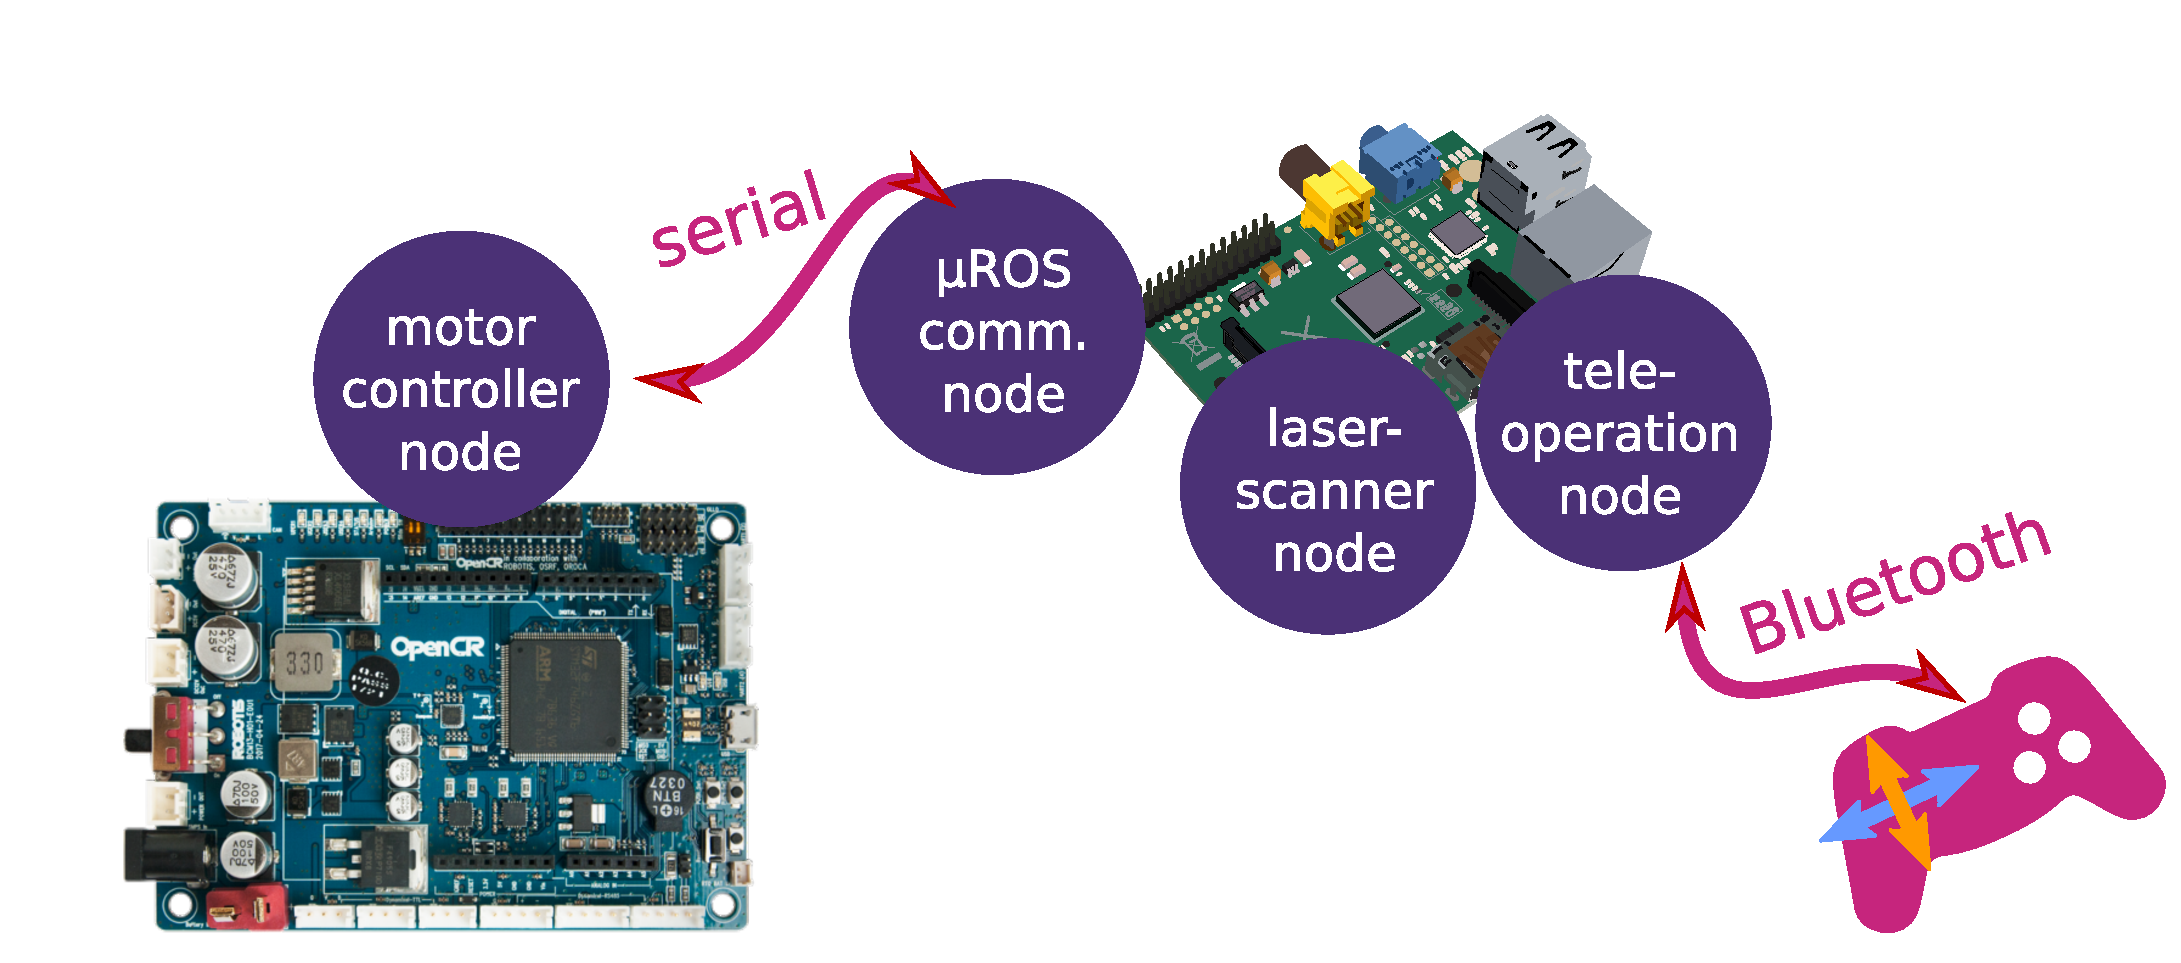
\includegraphics[width=.9\textwidth]{./figures/ros_nodes_on_robots.pdf}
      \end{figure}
  \end{frame}
  
  \begin{frame}[plain]{Nodes}{Where should a node run?}
    % So your biggest problem is that you have all these different parts of a robot that need to exchange data with each other. This is exactly where ROS can help you. ROS 2 uses the "Data Distribution Service" or DDS for short. DDS manages the network communication between the ROS-nodes automatically.
    \textbf{ROS without a robot!}
      \begin{figure}[tbh!]
        \centering
        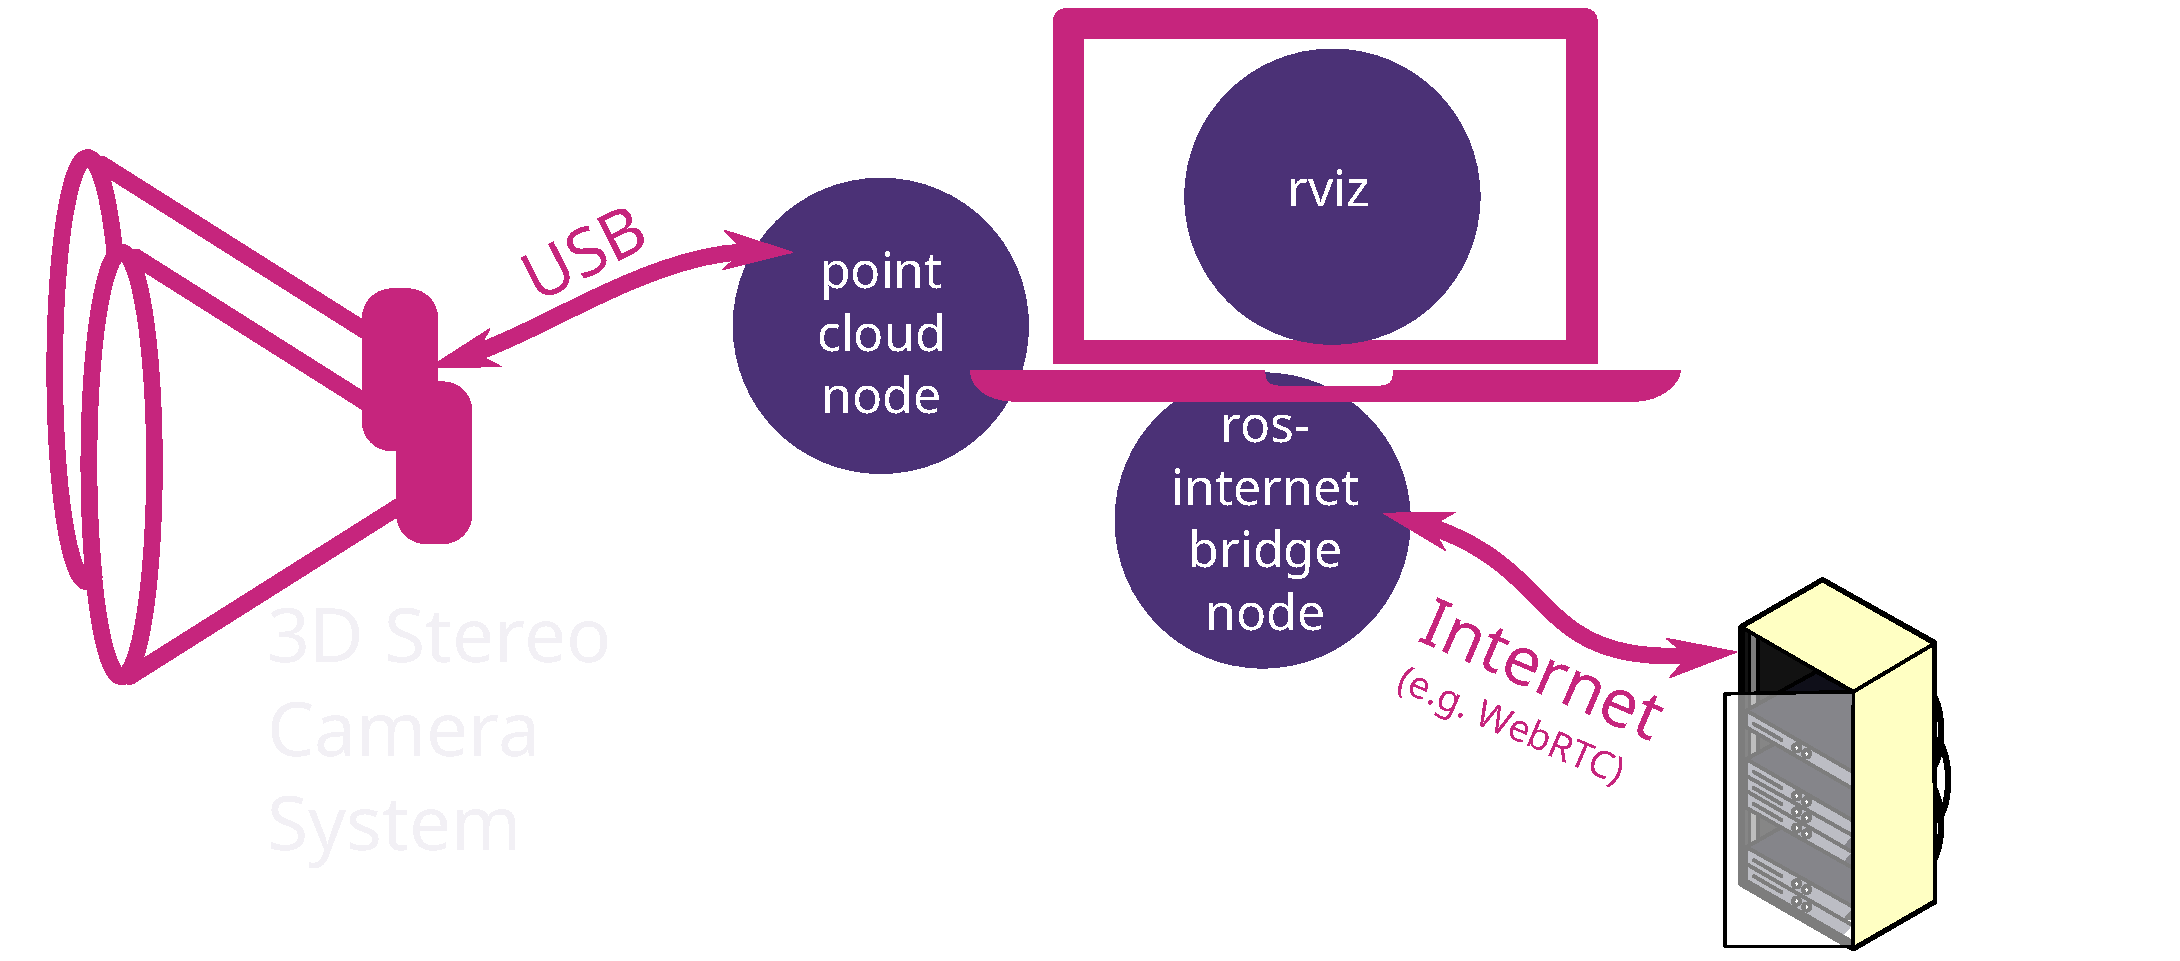
\includegraphics[width=.9\textwidth]{./figures/ros_nodes_example_3.pdf}
      \end{figure}

  \end{frame}



\begin{frame}{Robotics for everyone}
    \centering
      Robotics gets complex quickly!\\
      \pause
      
      \vspace{1em}
      Why not let AI generate code for it?
  
      \begin{minipage}{0.6\textwidth}
          \begin{alertblock}{
\includegraphics[height=1em]{figures/hare_head_darkmode.pdf} Warning!}
              Vibe-code machines that manipulate things in the real world is a very bad idea!
          \end{alertblock}
  \end{minipage}

  \vspace{1em}
  $\Rightarrow$ ROS is a good start but we need more\\tools to make it usable for everyone!
\end{frame}
  

\begin{frame}{Configure robots}
    \begin{minipage}{0.45\textwidth}
        \begin{block}{}
            1. Select components\\
            \tiny $\rightarrow$ This should also define the \textbf{capabilties} of the system.
        \end{block}
        \begin{minipage}{0.27\textwidth}
            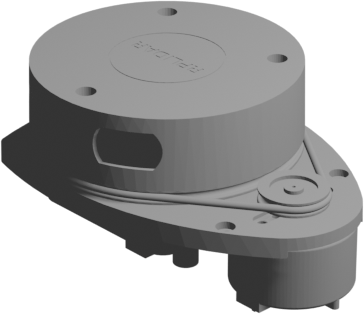
\includegraphics[height=1.2cm]{figures/rplidar.png}\\
            \small
            RPLidar
        \end{minipage} + \begin{minipage}{0.27\textwidth}
            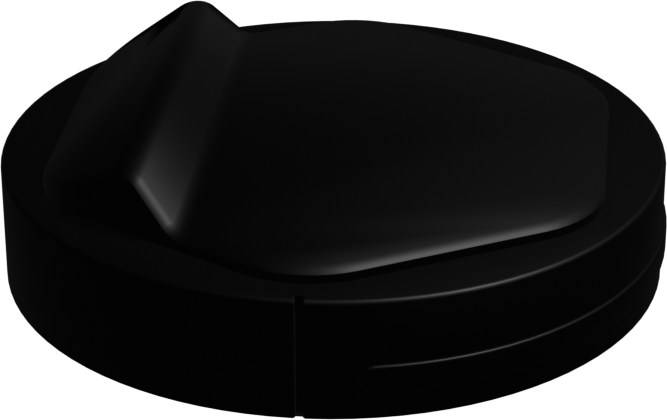
\includegraphics[height=1.2cm]{figures/kobuki_base.png}\\
            \small
            Kobuki Base
        \end{minipage} + \begin{minipage}{0.27\textwidth}
            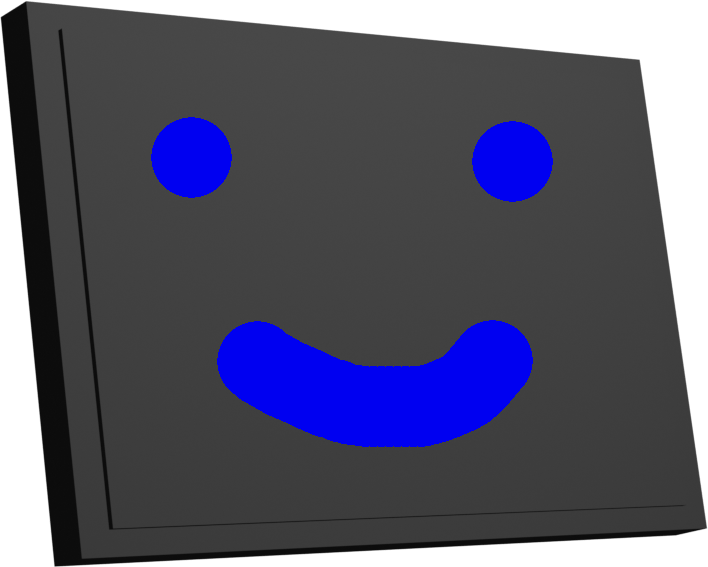
\includegraphics[height=1.2cm]{figures/display.png}\\
            \small
            Display
        \end{minipage}
        \vspace{1em}\\
        \tiny URDF-Editor: \url{https://brean.github.io/urdf-editor/}
    \end{minipage}\begin{minipage}{0.07\textwidth}
        \hspace{0.1cm}
    \end{minipage}\begin{minipage}{0.45\textwidth}
        \begin{block}{}
            2. Annotate environment\\
            \tiny $\rightarrow$ place waypoints, areas, paths in a map.
        \end{block}
        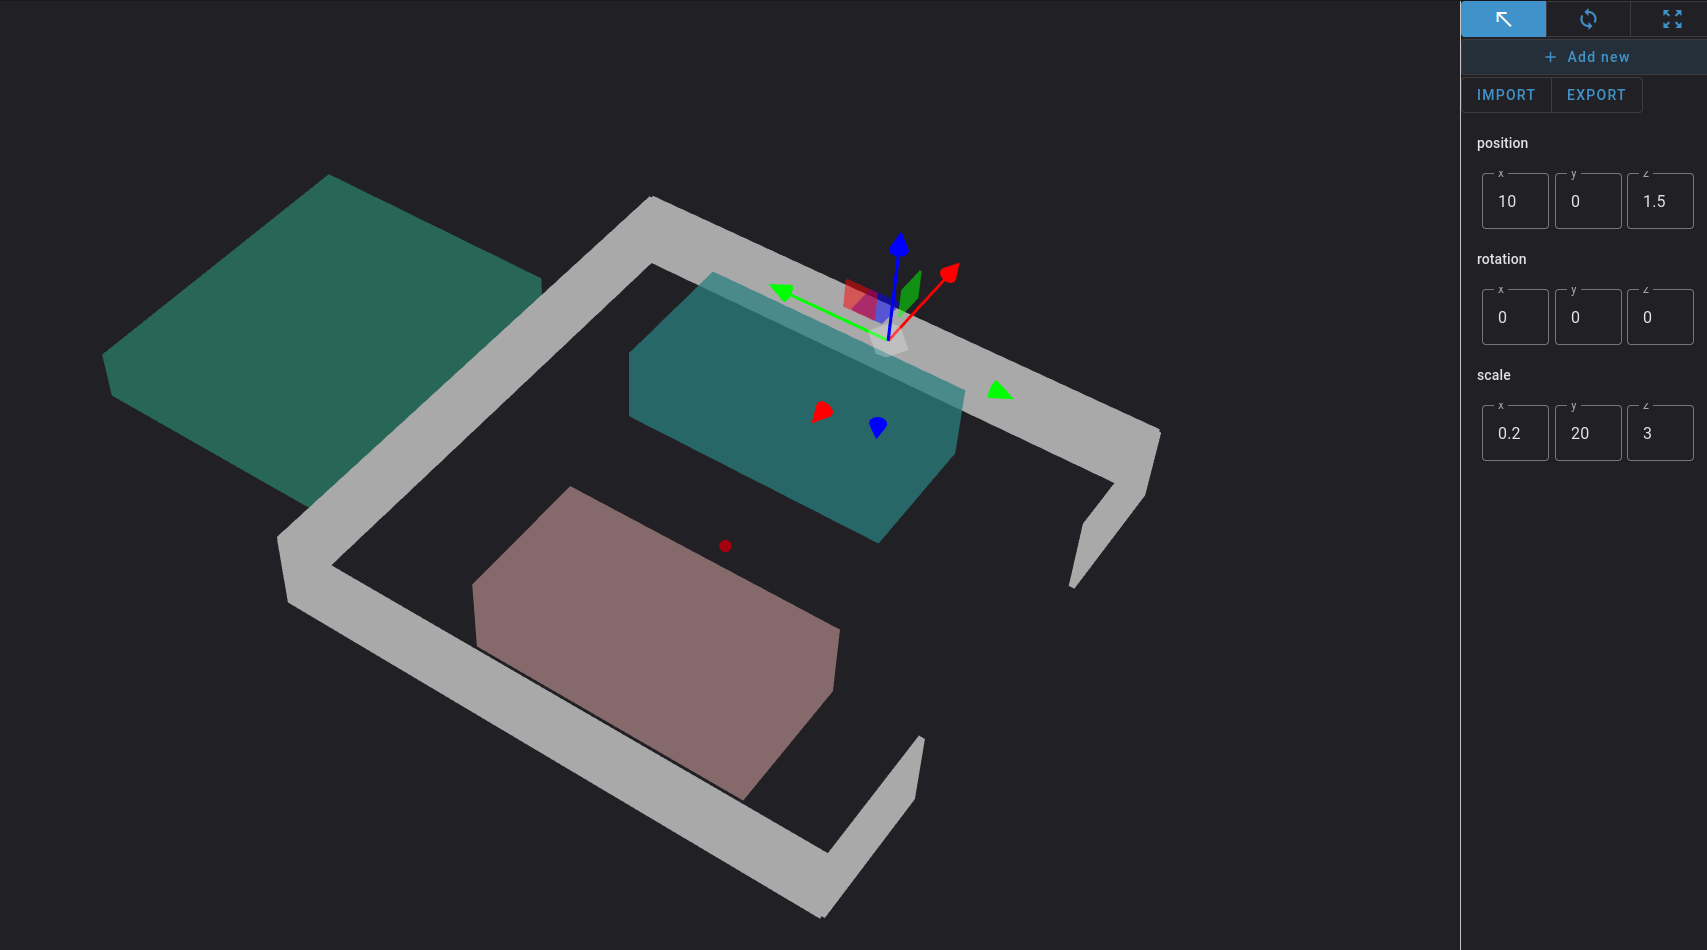
\includegraphics[height=3.5cm]{figures/map_editor_basic_scene.png}\\
        \tiny map-editor
    \end{minipage}
\end{frame}

\begin{frame}{Configure robots}
    \begin{minipage}{0.45\textwidth}
    \begin{block}{}
        3. Define some behavior\\
        \tiny $\rightarrow$ AI: simple Logic all the way to Schwarm intelligence.
    \end{block}
        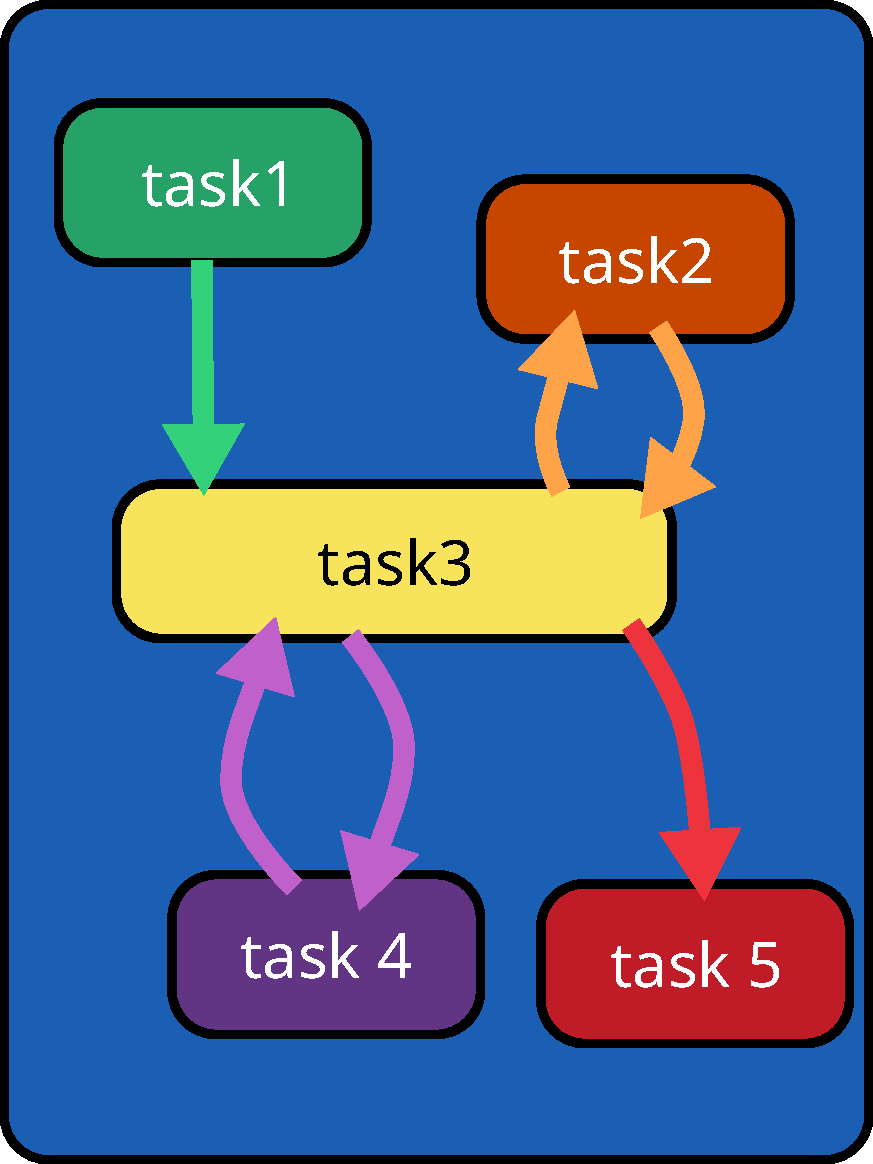
\includegraphics[height=5cm]{figures/planning_graph.pdf}\\
        \tiny
        (simple state machine/behavior graph)
    \end{minipage}\begin{minipage}{0.06\textwidth}
        \hspace{.1cm}
    \end{minipage}\begin{minipage}{0.45\textwidth}
    \begin{block}{}
        4. Deployment: Simulation / Deployment\\
        \tiny $\rightarrow$ compile and deploy
    \end{block}
        
\includegraphics[height=5cm]{figures/launch.pdf}
    \end{minipage}
\end{frame}

% Use AI to create complex setups from recipes
% More tools for generating code (e.g. low level-driver for MicroROS to control motors, similar to how you configure a Linux kernel)

% Include safety and IT-security

% Commercial 
\begin{frame}{Open Door Day 2025}{Visit me at work!}
    \centering
    \textbf{5. September 2025} at DFKI RIC, Robert-Hooke-Str. 1, 28359 Bremen

    \movie[height=0.7\textheight, loop, autostart=true] {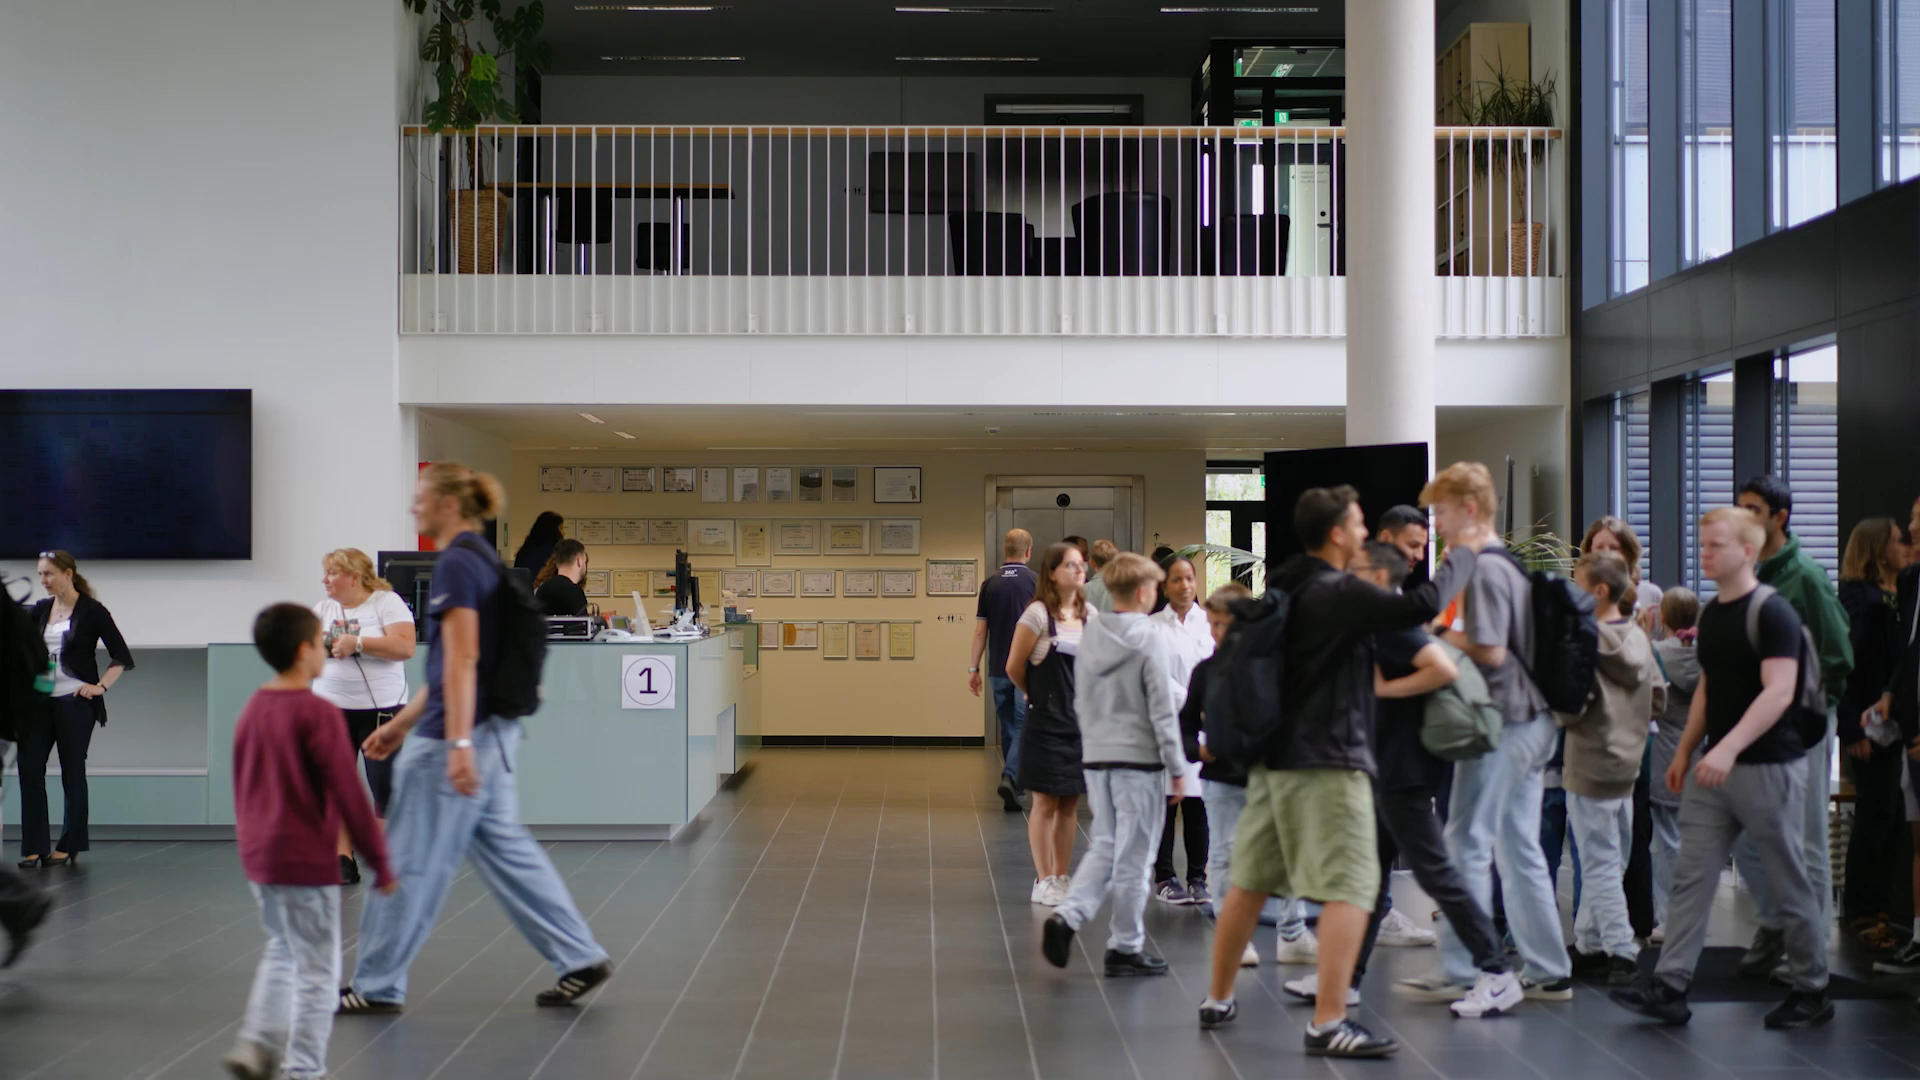
\includegraphics[height=0.7\textheight]{video/tdot.png}}{video/tdot.mkv}

    \url{https://robotik.dfki-bremen.de}
\end{frame}

% \begin{frame}{My next talk}
%   \centering
%   Chaos Communication Congress 2025
  
%   Building a robot that can survive the lunar night!

%   
\includegraphics[width=0.3\textwidth]{figures/samler-logo.png}
% \end{frame}
\end{document}